\section{Lesson 13 --- 19/11/2026}

\subsection{BIRCH}

At the end of the last lesson we saw that the main limitation of hierarchical clustering is its cost: distance-matrix implementations need $O(n^2)$ memory and repeated scans of the data. Modern variants keep the hierarchical reasoning but address scale. \g{BIRCH} (\s{Balanced Iterative Reducing and Clustering using Hierarchies}) is one of them: it compresses the data incrementally into a \g{Clustering Feature tree} (CF-tree) and controls memory through compact summaries.

\subsubsection{The scalability problem and the BIRCH idea}

The problem BIRCH addresses is the following:
\begin{itemize}
  \item very large numerical datasets may not fit into main memory;
  \item many hierarchical algorithms repeatedly scan the data;
  \item disk I/O can dominate the clustering time.
\end{itemize}
The idea is to replace many raw points with compact, incrementally updated cluster summaries:
\begin{enumerate}
  \item summarize the points using CF statistics;
  \item organize the summaries in a compact CF-tree;
  \item cluster the summaries rather than all the points.
\end{enumerate}
Typically one scan of the dataset is enough to build the CF-tree, and the time is near-linear for bounded tree parameters.

\subsubsection{Clustering features}

A clustering feature summarizes a subcluster without storing its individual observations.

\begin{definition}[Clustering feature]
Let $C = \{x_1, \dots, x_N\}$ be a subcluster of $d$-dimensional points. Its \g{clustering feature} is the triple
\[
CF(C) = (N, LS, SS), \qquad N = |C|, \quad LS = \sum_{i=1}^{N} x_i, \quad SS = \sum_{i=1}^{N} x_i^2,
\]
where $N$ counts the observations, the \g{linear sum} $LS$ is a vector used to recover the centroid, and the \g{square sum} $SS$ contains, for each dimension, the sum of the squared coordinates (the per-dimension second moments, useful for compactness).
\end{definition}

The key property is \g{additivity}: for two disjoint subclusters $A$ and $B$,
\[
CF(A \cup B) = CF(A) + CF(B),
\]
since each statistic can be updated by simple addition. So cluster summaries can be merged without accessing the underlying data points, and CFs preserve exactly what BIRCH needs for compactness checks and hierarchical aggregation.

\begin{example}
Cluster 1 contains the three points $(2,5)$, $(3,2)$, $(4,3)$. Then $N = 3$, $LS = (2+3+4,\ 5+2+3) = (9,10)$ and $SS = (4+9+16,\ 25+4+9) = (29,38)$, so
\[
CF_1 = (3, (9,10), (29,38)).
\]
Cluster 2 contains three more points and is summarized directly by $CF_2 = (3, (35,36), (417,440))$. The combined cluster of six points is
\[
CF_1 + CF_2 = (6, (44,46), (446,478)).
\]
\end{example}

From a CF we can compute the centroid, the radius and the diameter of the subcluster:
\begin{itemize}
  \item \g{centroid}: the mean vector of the subcluster,
  \[
  \mu = \frac{LS}{N};
  \]
  \item \g{radius}: the root-mean-squared distance of the points from $\mu$,
  \[
  R = \sqrt{\frac{SS}{N} - \norm{\frac{LS}{N}}^2};
  \]
  \item \g{diameter}: the root-mean-squared pairwise distance (for $N > 1$),
  \[
  D = \sqrt{\frac{2N \cdot SS - 2\norm{LS}^2}{N(N-1)}}.
  \]
\end{itemize}
In $R$ and $D$, $SS$ stands for the sum of its components over all the dimensions, i.e.\ $\sum_i \norm{x_i}^2$.

\begin{remark}
The slides store $SS$ per dimension, e.g.\ $(29,38)$, while the book (Han, Pei, Tong, Ex.~8.5) stores it as a scalar: $CF_1 = \langle 3, (9,10), 67 \rangle$ and $CF_1 + CF_2 = \langle 6, (44,46), 924 \rangle$. The two are consistent, since $29 + 38 = 67$ and $446 + 478 = 924$; in the formulas for $R$ and $D$ the scalar version is the one to use. The book also calls $R$ and $D$ ``average'' distances, but they are root-mean-square distances.
\end{remark}

\subsubsection{The CF-tree}

The CF-tree is a compact hierarchy that stores nested summaries of subclusters in memory. Its key properties are:
\begin{itemize}
  \item it is a \g{height-balanced} hierarchical index;
  \item \g{non-leaf} (internal) entries point to child nodes and store routing summaries: the CF of a parent entry is the sum of the CFs of the entries in the corresponding child node,
  \[
  CF(\text{parent entry}) = \sum CF(\text{entries in the child node});
  \]
  \item \g{leaf} entries represent compact subclusters, the \g{microclusters};
  \item leaves are linked for sequential traversal.
\end{itemize}
Note that a leaf node holds several CF entries: it is not necessarily one cluster.

The structure is controlled by two capacity limits and one compactness threshold:
\begin{itemize}
  \item $B$, \g{branching factor}: maximum number of entries (children) in a non-leaf node;
  \item $L$, \g{leaf capacity}: maximum number of CF entries stored in a leaf node;
  \item $T$, \g{compactness threshold}: maximum permitted diameter of a leaf-entry subcluster.
\end{itemize}
$B$ and $L$ control the size of the tree, while $T$ controls the granularity of the microclusters.

\begin{remark}
The book introduces only the parameters $B$ and $T$; the slides add the leaf capacity $L$, as in the original BIRCH paper.
\end{remark}

\subsubsection{Inserting a point}

Each new point is inserted by choosing the nearest entry and then checking compactness and capacity:
\begin{enumerate}
  \item \g{descend the tree}: at each non-leaf node, choose the closest CF entry;
  \item \g{choose a leaf entry}: identify the closest subcluster in the selected leaf;
  \item \g{test the updated diameter}: can the new point be absorbed while keeping $D \le T$?
  \begin{itemize}
    \item if yes, absorb the point (update $N$, $LS$ and $SS$) and update the leaf CF and all the ancestor summaries;
    \item if no and the leaf has room, create a new CF entry for the point;
    \item if no and the leaf is full, split the leaf and update the parent; splits may propagate and create a new root.
  \end{itemize}
\end{enumerate}
``Closest'' only identifies a candidate: it does not override the threshold $T$ or the leaf capacity $L$.

When a leaf overflows, it is split as follows:
\begin{enumerate}
  \item \g{find split seeds}: choose the two farthest CF entries as seeds for two new leaves;
  \item \g{redistribute entries}: assign the other entries (including the new point) to the nearest seed;
  \item \g{update aggregated CFs}: recompute the parent entries from the updated children;
  \item \g{propagate if necessary}: split a full parent; splitting the root increases the height of the tree.
\end{enumerate}
Only the compact CF summaries need to move during restructuring, not the original data points.

\begin{example}[Building a CF-tree]
We insert six points $x_1, \dots, x_6$ one at a time, with leaf capacity $L = 3$ (an illustrative value).
\begin{enumerate}
  \item $x_1$ creates the first entry $CF_1$ of the root leaf. Adding $x_2$ would make the diameter exceed $T$, so a second entry $CF_2$ is created: the closest subcluster is not necessarily allowed to absorb the point. The leaf now stores two CF entries, one for $\{x_1\}$ and one for $\{x_2\}$.
  \item $x_3$ is closest to $CF_1$, but merging it would exceed $T$: distance selects a candidate, the threshold decides whether insertion is allowed. We create $CF_3$ for $\{x_3\}$, and the leaf now holds $L = 3$ entries.
  \item $x_4$ is closest to $CF_2$ and the diameter stays within $T$, so $CF_2$ absorbs it, and its ancestors' summaries are updated.
  \item $x_5$ cannot be absorbed while satisfying $T$, and the leaf already holds $L = 3$ entries: creating a fourth entry requires a leaf split. The entries are redistributed into two leaves, $\{CF_1, CF_3\}$ and $\{CF_5, CF_2\}$, where $CF_5$ summarizes $\{x_5\}$. A new non-leaf root with entries $CF_A = CF_1 + CF_3$ and $CF_B = CF_5 + CF_2$ is created: splitting the root increased the height of the tree by one.
  \item $x_6$ descends through $CF_A$ and joins the subcluster represented by $CF_3$, since the diameter remains $\le T$.
\end{enumerate}
The final tree is
\begin{center}
\begin{tikzpicture}[
  node distance=0.6cm and 1.2cm,
  box/.style={draw, rounded corners, minimum height=0.7cm, inner sep=4pt, font=\small},
  every node/.append style={font=\small}]
  \node[box] (root) {$CF_A \mid CF_B$};
  \node[box, below left=0.9cm and 0.6cm of root] (l1) {$CF_1 \mid CF_3$};
  \node[box, below right=0.9cm and 0.6cm of root] (l2) {$CF_5 \mid CF_2$};
  \node[below=0.3cm of l1] {$\{x_1\} \quad \{x_3, x_6\}$};
  \node[below=0.3cm of l2] {$\{x_5\} \quad \{x_2, x_4\}$};
  \node[right=0.3cm of root, gray] {non-leaf root};
  \draw[-{Latex}] (root) -- (l1);
  \draw[-{Latex}] (root) -- (l2);
  \draw[dashed, {Latex}-{Latex}] (l1) -- node[above, gray] {leaf link} (l2);
\end{tikzpicture}
\end{center}
The CF-tree is built incrementally, without storing every raw point.
\end{example}

\subsubsection{The four phases of BIRCH}

Inserting points builds microclusters online; the overall partition is obtained and refined in later phases. The first pass compresses the data, and the subsequent stages can improve the partition:
\begin{enumerate}
  \item \g{Phase 1, build the initial CF-tree} (mandatory): a single sequential pass over the data, keeping the tree in memory;
  \item \g{Phase 2, condense the CF-tree} (optional): build a smaller tree, for example by increasing $T$, and optionally remove or handle outliers;
  \item \g{Phase 3, global clustering} (core): apply a global clustering algorithm to the leaf CF summaries, to produce higher-level clusters;
  \item \g{Phase 4, refine assignments} (optional): scan the original dataset again to label the individual points, refine the boundaries and reconsider outliers.
\end{enumerate}
So compression (the CF-tree) and final partitioning are distinct tasks. For instance, phase 3 can use one of the partitioning or agglomerative algorithms we have already seen, now applied to a few microclusters instead of $n$ points.

During phase 1, BIRCH has to stay within its memory budget. It can do so by rebuilding a smaller CF-tree without rescanning the raw dataset:
\begin{enumerate}
  \item \g{start}: choose an initial $T$ and insert the objects one by one;
  \item \g{monitor}: check whether the in-memory CF-tree is becoming too large;
  \item \g{rebuild}: if so, increase $T$ and build a more compact tree from the old leaf CFs;
  \item \g{continue}: resume insertion until the full dataset has been scanned.
\end{enumerate}
Rebuilding works on the existing CF summaries, so there is no need to reread the input objects. Outlier handling can be included during condensation or refinement.

\subsubsection{Strengths and limitations}

BIRCH is a scalable method with clear assumptions and trade-offs.
\begin{center}
\begin{tabular}{@{}p{7cm}p{7cm}@{}}
\toprule
Strengths & Limitations \\
\midrule
Designed for large numerical datasets. & Uses numerical features and distance-based compactness. \\
Typically requires just one pass to construct the initial CF-tree. & Sensitive to the insertion order and to the choice of $T$. \\
Compact summaries reduce memory and I/O costs. & Radius and diameter criteria tend to favor roughly spherical microclusters. \\
\bottomrule
\end{tabular}
\end{center}
The cost is approximately $O(n)$ for bounded tree height and entry capacities. In short, BIRCH trades exact raw-data storage for scalable, hierarchy-based compression. Its preference for spherical clusters is the motivation for the next family of methods, the density-based algorithms, which can find clusters of arbitrary shape.


\subsection{Density-based clustering methods}

We change the point of view again: the main idea is to discover clusters not through the distance from a representative, but through \g{density}. We look for dense regions separated by areas of lower density. If we build clusters by following the density, through connectivity, they do not need to have a spherical shape: they can have any shape, even non-convex. To run any of these algorithms we have to tell it what our idea of density is and how we define a high-density region. The number of clusters is not given in advance: it depends on how we define high density and it emerges from the data. Points outside the dense regions can be labelled as noise.

There are several methods, which differ in how they model density:
\begin{itemize}
  \item \g{DBSCAN} uses one density threshold;
  \item \g{OPTICS} and \g{HDBSCAN} explore several density levels;
  \item \g{DENCLUE} uses density estimation;
  \item \g{CLIQUE} uses grids and subspaces.
\end{itemize}
In all of them the distance metric and the feature scales define what ``local'' means.

\subsubsection{DBSCAN}

In \g{DBSCAN} (\s{Density-Based Spatial Clustering of Applications with Noise}) we use a threshold as density, defined by two parameters: $\varepsilon$, the \g{neighbourhood radius}, and $MinPts$, the minimum neighbourhood count, including the point itself.

\begin{definition}[$\varepsilon$-neighbourhood and core point]
The \g{$\varepsilon$-neighbourhood} of a point $p$ in the dataset $D$ is
\[
N_\varepsilon(p) = \{q \in D : dist(p, q) \le \varepsilon\}.
\]
A point $p$ is a \g{core point} if $|N_\varepsilon(p)| \ge MinPts$.
\end{definition}

Note that the condition is ``at least $MinPts$'' and that the query point itself is counted. With these two notions we need to introduce some definitions:
\begin{itemize}
  \item \g{Direct density reachability}: $p$ is directly density-reachable from $q$ when $p \in N_\varepsilon(q)$ and $q$ is a core point. The direction matters: the source must be core, while the destination may be core or border, so the relation need not be symmetric.
  \item \g{Density reachability}: $p$ is density-reachable from $q$ if there is a chain $q = p_1, \dots, p_t = p$ where $p_{i+1}$ is directly density-reachable from $p_i$ at every step. Every point that starts a step must be core, while the final point may be a border point.
  \item \g{Density connectivity}: $p$ and $q$ are density-connected if some point $o$ can density-reach both of them, i.e.\ they share a common core origin in the same dense region.
\end{itemize}

\begin{remark}
Only a core point can propagate a cluster to its neighbours. Density reachability can connect points much farther apart than $\varepsilon$. Density connectivity is symmetric, while density reachability need not be.
\end{remark}

\begin{example}
Let $MinPts = 3$, and let $m$ and $p$ be core points while $q$ is not, with $q \in N_\varepsilon(m)$ and $m$, $p$ in each other's neighbourhood. Then $q$ is directly density-reachable from $m$, but not vice versa, while $m$ and $p$ are directly density-reachable from each other. Starting from $p$ we can reach $m$ and then $q$, so $q$ is density-reachable from $p$; starting from the non-core point $q$ we cannot expand towards $p$. Since $m$ density-reaches both $p$ and $q$, they are density-connected. If two dense regions are separated by a sparse gap with no chain of core points, they remain separate: a border point can end a chain, but cannot bridge two core components.
\end{example}

We can then define three kinds of points:
\begin{itemize}
  \item \g{core}: at least $MinPts$ points in its $\varepsilon$-neighbourhood;
  \item \g{border}: not core, but within $\varepsilon$ of a core point; it joins a cluster without expanding it;
  \item \g{noise}: neither core nor reachable from a core point. Noise is relative to the chosen parameters.
\end{itemize}
$MinPts$ is a local density threshold, not a requested cluster size.

\paragraph{Cluster expansion.} The algorithm grows each cluster from a core point:
\begin{enumerate}
  \item select an unprocessed point and query its $\varepsilon$-neighbourhood; if it is non-core, mark it as noise for now;
  \item if it is a core point, start a cluster: add its neighbours to a seed set and process the seed set until it is exhausted;
  \item expand only from core points: add the neighbourhood of every newly discovered core point, while border points join the cluster but do not expand it;
  \item continue until all the points are processed. A point previously marked as noise can later become a border point.
\end{enumerate}
Cluster growth stops when no new density-reachable points remain. With this algorithm we find clusters and outliers at the same time.

\begin{algorithm}[H]
\caption{DBSCAN}
\KwIn{a dataset $D$ of $n$ objects, the radius $\varepsilon$, the density threshold $MinPts$}
\KwOut{a set of density-based clusters}
mark all objects as unvisited\;
\Repeat{no object is unvisited}{
  randomly select an unvisited object $p$ and mark it as visited\;
  \eIf{$|N_\varepsilon(p)| \ge MinPts$}{
    create a new cluster $C$ and add $p$ to $C$\;
    let $N$ be the set of objects in $N_\varepsilon(p)$\;
    \ForEach{$p' \in N$}{
      \If{$p'$ is unvisited}{
        mark $p'$ as visited\;
        \lIf{$|N_\varepsilon(p')| \ge MinPts$}{add the points of $N_\varepsilon(p')$ to $N$}
      }
      \lIf{$p'$ is not yet a member of any cluster}{add $p'$ to $C$}
    }
    output $C$\;
  }{
    mark $p$ as noise\;
  }
}
\end{algorithm}

\begin{remark}
The slides define clusters with the original DBSCAN notions (direct density reachability, border points assigned during expansion) and show the pseudocode of the book (Fig.~8.18). The book instead explains the variant DBSCAN$^*$, where a cluster is a maximal set of density-connected core objects and border objects are attached in post-processing.
\end{remark}

\paragraph{Computational cost.} The main cost is in the neighbourhood queries:
\begin{itemize}
  \item a standard sequential implementation queries each point at most once, but a single outer scan does not imply a linear total running time;
  \item \g{without an effective spatial index}, scanning all the points for every neighbourhood gives $O(n^2)$ distance checks, and the cost of the distance function must be included in the total time;
  \item with an \g{effective index}, for favourable low-dimensional data and sufficiently small neighbourhoods the runtime can approach $O(n \log n)$, but the worst case remains quadratic;
  \item \g{memory}: on-demand neighbourhood queries avoid storing all pairwise distances, while implementations that cache all neighbourhoods can require $O(n^2)$ memory.
\end{itemize}

Compared with a medoid-based partitioning method such as CLARANS, DBSCAN can follow connected, non-convex regions and leave isolated points unassigned. These examples illustrate the behaviour of the two methods; they are not a universal ranking.

\paragraph{One density threshold can be insufficient.} DBSCAN uses a single global density level, and sometimes this is not enough:
\begin{itemize}
  \item with a \g{large $\varepsilon$}, sparse structures may connect, merging different regions;
  \item with a \g{small $\varepsilon$}, dense groups remain, while sparse groups may fragment or become noise.
\end{itemize}
So a single $(\varepsilon, MinPts)$ pair may not recover all the clusters when the densities differ substantially, and parameter tuning cannot always resolve a mismatch with the model. Moreover, the result is sensitive to $\varepsilon$: with $MinPts$ fixed, reducing $\varepsilon$ raises the required local density, and clusters may split, shrink or disappear. Small parameter changes can produce large changes near a connectivity threshold, so we should inspect more than the cluster count: cluster sizes, noise fraction and connectivity (thin chains of core points can merge otherwise separate regions).

Different densities are a limitation of the model itself, and they are addressed by methods that explore several density levels, such as OPTICS and HDBSCAN, which we will see later. Before that, we still need a way to choose the \s{one} pair $(\varepsilon, MinPts)$ that DBSCAN requires.

\paragraph{The k-distance heuristic.} The \g{k-distance heuristic} is a heuristic method to set $\varepsilon$ once $MinPts$ is fixed. It does not solve the problem of different densities: it only helps to pick a reasonable single threshold.

\begin{definition}[k-distance]
Let $d_k(p)$ be the distance from $p$ to its $k$-th nearest \s{other} point. Since $MinPts$ includes $p$ itself, we use $k = MinPts - 1$. With this convention,
\[
p \text{ is a core point} \iff d_k(p) \le \varepsilon.
\]
\end{definition}
For example, if a point has four other neighbours within $\varepsilon$, then for $k = 4$ we use $MinPts = 5$. We should always state whether the point itself is included in the neighbour rank.

\paragraph{Choosing $\varepsilon$ from a sorted k-distance plot.} The equivalence above suggests how to choose $\varepsilon$:
\begin{enumerate}
  \item choose $MinPts$ and compute $d_k(p)$ for every point, with $k = MinPts - 1$;
  \item sort the distances (here in descending order) and plot them against the point rank;
  \item inspect the change in slope: the high-distance tail contains the sparse points, and the transition (the \g{knee}) suggests candidate values of $\varepsilon$.
\end{enumerate}
In the example of the slides the knee is at $\varepsilon = 0.28$.

\begin{center}
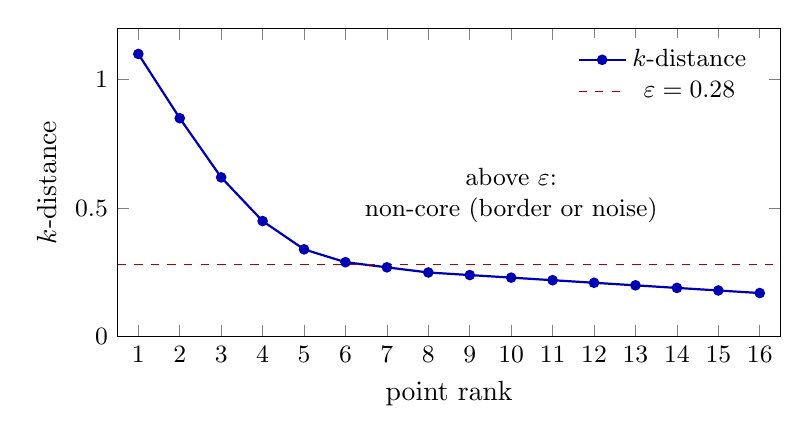
\begin{tikzpicture}
\begin{axis}[
  width=10cm, height=5.5cm,
  xlabel={point rank}, ylabel={$k$-distance},
  xmin=0.5, xmax=16.5, ymin=0, ymax=1.2,
  xtick={1,...,16}, ticklabel style={font=\small},
  legend style={font=\small, draw=none}, legend pos=north east]
  \addplot[thick, mark=*, mark size=1.5pt, blue!70!black] coordinates {
    (1,1.10) (2,0.85) (3,0.62) (4,0.45) (5,0.34) (6,0.29) (7,0.27) (8,0.25)
    (9,0.24) (10,0.23) (11,0.22) (12,0.21) (13,0.20) (14,0.19) (15,0.18) (16,0.17)};
  \addlegendentry{$k$-distance}
  \addplot[dashed, red!70!black, domain=0.5:16.5] {0.28};
  \addlegendentry{$\varepsilon = 0.28$}
  \node[font=\small, align=center] at (axis cs:10,0.55) {above $\varepsilon$:\\ non-core (border or noise)};
\end{axis}
\end{tikzpicture}
\end{center}

\begin{remark}
The values in the figure are illustrative, only the shape and the threshold $\varepsilon = 0.28$ follow the slides. The points above $\varepsilon$ are non-core, but they may still be border points: the plot proposes candidate thresholds, it does not identify noise exactly. Moreover, the knee may be weak, multiple or absent.
\end{remark}

\paragraph{Choosing $MinPts$.} The k-distance plot needs $MinPts$ as input, which is chosen with some rules of thumb:
\begin{itemize}
  \item \g{dimension-based starting values}: for $d$ meaningful numeric dimensions, $MinPts \ge d + 1$ and $MinPts \approx 2d$ are common starting heuristics;
  \item \g{explore a small range}: for $d = 2$, try values such as $4$, $6$, $8$ and $12$; larger values demand stronger local support and often suppress small groups;
  \item \g{choose the representation first}: scale the features when their units should not determine the distance, select a meaningful metric and remove irrelevant dimensions;
  \item \g{validate the result}: increase $MinPts$ when apparent clusters rely on weak local support; the dimension-based rules are not guarantees.
\end{itemize}
So $MinPts$ is selected jointly with $\varepsilon$, after choosing the metric and the preprocessing.
